\documentclass[11pt]{preprint}

\setlength{\topmargin}{0mm} \setlength{\oddsidemargin}{0mm}
\setlength{\textwidth}{160mm} \setlength{\textheight}{215mm}

\usepackage{amssymb,amsmath,amscd,amsthm}
\usepackage{graphics}
\usepackage{tikz}

\def\enumb{\begin{enumerate}}
\def\enume{\end{enumerate}}
\def\itemb{\begin{itemize}}
\def\iteme{\end{itemize}}
\def\integers{\mathbb{Z}}

\def\multiset#1#2{\ensuremath{\left(\kern-.3em\left(\genfrac{}{}{0pt}{}{#1}{#2}\right)\kern-.3em\right)}}



\newtheorem{proposition}{Proposition}
\newtheorem{theorem}{Theorem}

\title{Discrete Mathematics, 2016 Spring - Worksheet 24}
\author{Instructor: Zsolt Pajor-Gyulai, CIMS}



\begin{document}

\maketitle

In all of the above problems explain your answer in full English sentences.

\enumb
\item The following picture represents a graph. Please write it as a pair of set $(V,E)$.
\begin{figure}[ht]
\centering
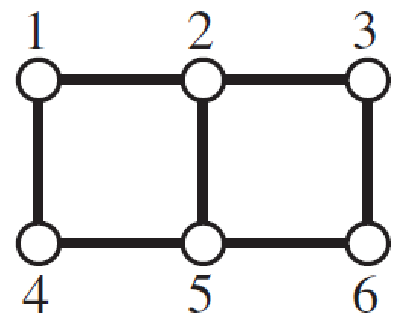
\includegraphics[scale=0.5]{WSGraph.pdf}
\end{figure}\vspace{-0.6cm}
\item Draw a picture of the following graph.
\[
\left(\{a,b,c,d,e\},\left\{\{a,b\},\{a,c\},\{a,d\},\{b,e\},\{c,d\}\right\}\right)
\]
\item Let $G$ be a graph in the figure. Draw pictures of the following subgraphs.

\begin{figure}[ht]
\centering
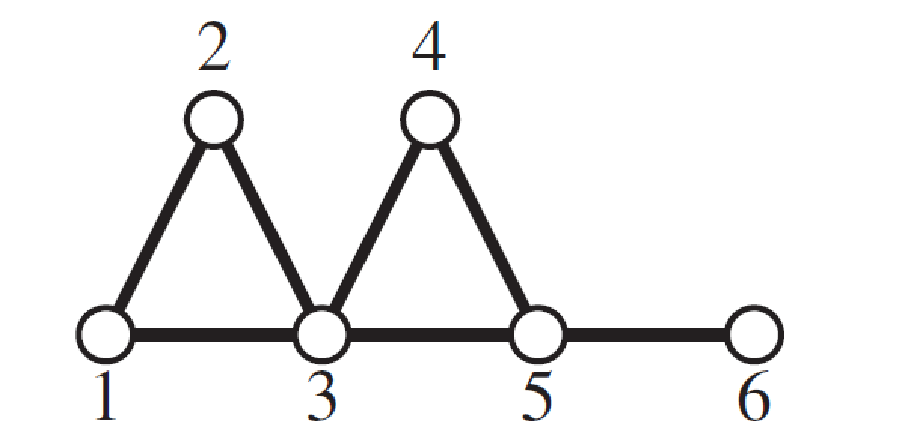
\includegraphics[scale=0.35]{Worksheet2.pdf}
\end{figure}\vspace{-0.9cm}
\enumb
\item $G-\{3\}$.
\item $G-\{5,6\}$
\item $G[\{2,4,6\}]$
\item $G[\{1,2,4,5\}]$.
\enume
\item Let $G$ be the graph in the picture.
\begin{figure}[ht]
\centering
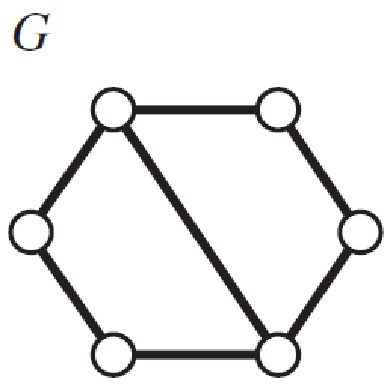
\includegraphics[scale=0.36]{Worksheet3.pdf}
\end{figure}
\enumb
\item Draw the complement graph $\bar{G}$.
\item Find $\alpha(G)$ and $\omega(G)$.
\enume\newpage
\item Prove the following proposition. (Proposition 48.13)
\begin{proposition}
Let $G$ be a graph with at least six vertices. Then $\omega(G)\geq 3$ or $\omega(\bar{G})\geq 3$.
\end{proposition}
\enume
\end{document}